\documentclass[10pt,a4paper]{article}
\usepackage[utf8]{inputenc}
\usepackage[T1]{fontenc}
\usepackage[spanish,provide=*]{babel}
\usepackage{mathptmx}
\usepackage[scaled=0.92]{helvet}
\usepackage[margin=1.9cm,top=1.8cm,bottom=1.9cm]{geometry}
\usepackage{graphicx}\usepackage{booktabs,graphicx,amsmath,amssymb,multirow,tabularx,float,enumitem,microtype}
\usepackage[table]{xcolor}
\usepackage[font=small,labelfont=bf,skip=3pt]{caption}
\usepackage{titlesec,fancyhdr}
\usepackage[hidelinks]{hyperref}
\definecolor{acc}{HTML}{2A78D6}
\titleformat{\section}{\large\bfseries\sffamily\color{acc}}{\thesection}{0.6em}{}
\titleformat{\subsection}{\normalsize\bfseries\sffamily}{\thesubsection}{0.5em}{}
\titlespacing*{\section}{0pt}{8pt}{3pt}
\titlespacing*{\subsection}{0pt}{6pt}{2pt}
\setlist{nosep,leftmargin=1.2em}
\setlength{\parskip}{2pt}
\pagestyle{fancy}\fancyhf{}
\lhead{\small\sffamily EDA 2026-2 · Proyecto final · Grupo 3}
\rhead{\small\sffamily\thepage}
\renewcommand{\headrulewidth}{0.3pt}
\newcommand{\Oh}[1]{\ensuremath{O(#1)}}
\renewcommand{\arraystretch}{1.12}

\begin{document}
\begin{center}
{\sffamily\small UTEC — Maestría en Ciencia de Datos e Inteligencia Artificial · Estructuras de Datos y Algoritmos 2026-2 · Prof. Heider Sánchez}\\[4pt]
{\LARGE\bfseries\sffamily EcoStream: estructuras de datos avanzadas orquestadas\\[2pt] en un pipeline de data streams para comercio electrónico}\\[5pt]
{\sffamily Grupo 3 — Integrante 1 · Integrante 2 · Integrante 3 · Integrante 4}\\[2pt]
{\small\sffamily Repositorio: \texttt{proyecto-eda-grupo3} · Escenario B (comercio electrónico)}
\end{center}

\noindent\colorbox{acc!8}{\parbox{\dimexpr\linewidth-2\fboxsep}{\small
\textbf{Resumen.} Diseñamos, implementamos y evaluamos \textbf{EcoStream}, un pipeline de procesamiento de streams de comercio electrónico de diez etapas en el que cada etapa usa la
estructura de datos más adecuada y su salida alimenta a otra de forma verificable: cola FIFO, Merge Sort y búsqueda binaria, heap de prioridades, tabla hash, LRU y matriz
dispersa, B+Tree paginado en disco, KD-Tree, Bloom Filter y Count-Min Sketch para fraude, MinHash+LSH y HNSW para similitud, grafo de co-compra con PageRank y Louvain, y
un servicio con Trie, Top-$K$ y panel. Todas las estructuras son implementaciones propias en Python, validadas con 14 pruebas contra referencias. Con datasets de
$10^3$ a $10^7$ elementos mostramos que las complejidades teóricas se cumplen en log-log; que el Bloom Filter alcanza su FPR teórica (1.008\,\% frente a 1.004\,\%) con
52$\times$ menos memoria que un \texttt{set}; que MinHash+LSH responde $\sim$9\,000$\times$ más rápido que la fuerza bruta con $10^7$ conjuntos sin perder vecinos con
$J\ge0.5$; que HNSW es 54$\times$ más rápido que el KNN exacto con recall@10 = 0.989 en $10^6$ vectores; y que Louvain es más estable que Label Propagation y logra mayor
modularidad en el grafo real de co-compra (0.755 frente a 0.630). El pipeline procesa 10M eventos de punta a punta.
}}

\section{Contexto y motivación}
Una tienda en línea recibe un flujo continuo de vistas, búsquedas, carritos, pagos, compras, devoluciones y reseñas. Sobre ese flujo
el negocio necesita, con baja latencia: atender primero los pagos y las órdenes urgentes; consultar productos por clave y por rango;
detectar medios de pago o dispositivos señalados y ráfagas de intentos (\emph{card testing}) \emph{antes} de aprobar una orden;
recomendar productos relacionados y complementarios; e identificar comunidades de co-compra y productos influyentes para
\emph{cross-selling}. Ninguna estructura resuelve todo: cada requisito tiene una estructura óptima distinta y el valor del sistema
está en \textbf{orquestarlas} de modo que la salida de cada etapa sea la entrada real de otra. El escenario elegido es el
\textbf{B (comercio electrónico)}; el grafo de dominio tiene a los productos como nodos y una arista ponderada entre productos
comprados en la misma orden.

\textbf{Datos.} Como base estructural se adoptó el esquema del dataset público \emph{eCommerce behavior data from multi category store}
(REES46, Kaggle: \texttt{event\_time, event\_type, product\_id, category\_code, brand, price, user\_id, user\_session}); el repositorio incluye
un cargador (\texttt{rees46\_loader.py}) que alimenta el mismo pipeline con el CSV real. Siguiendo la recomendación del enunciado, el
componente de \emph{stream} se genera sintéticamente y de forma vectorizada (10M eventos en $\sim$20\,s) con propiedades controladas por semilla:
catálogo de 20\,000 productos en 40 categorías con popularidad Zipf, afinidad usuario$\to$categoría (comunidades reales) y categorías
complementarias plantadas; órdenes de 1–6 ítems con envío express/estándar/programado; 2\,\% de re-entregas duplicadas, 0.5\,\% de registros sucios
(tipo en mayúsculas, precio con coma decimal, faltante o negativo, categoría en mayúsculas); 500 tokens de pago comprometidos y ráfagas
de 25–80 intentos de pago en $\le$3 minutos, la mitad con tokens nuevos que solo una estimación de frecuencia puede detectar.

\section{Arquitectura del pipeline}
\begin{figure}[H]
\centering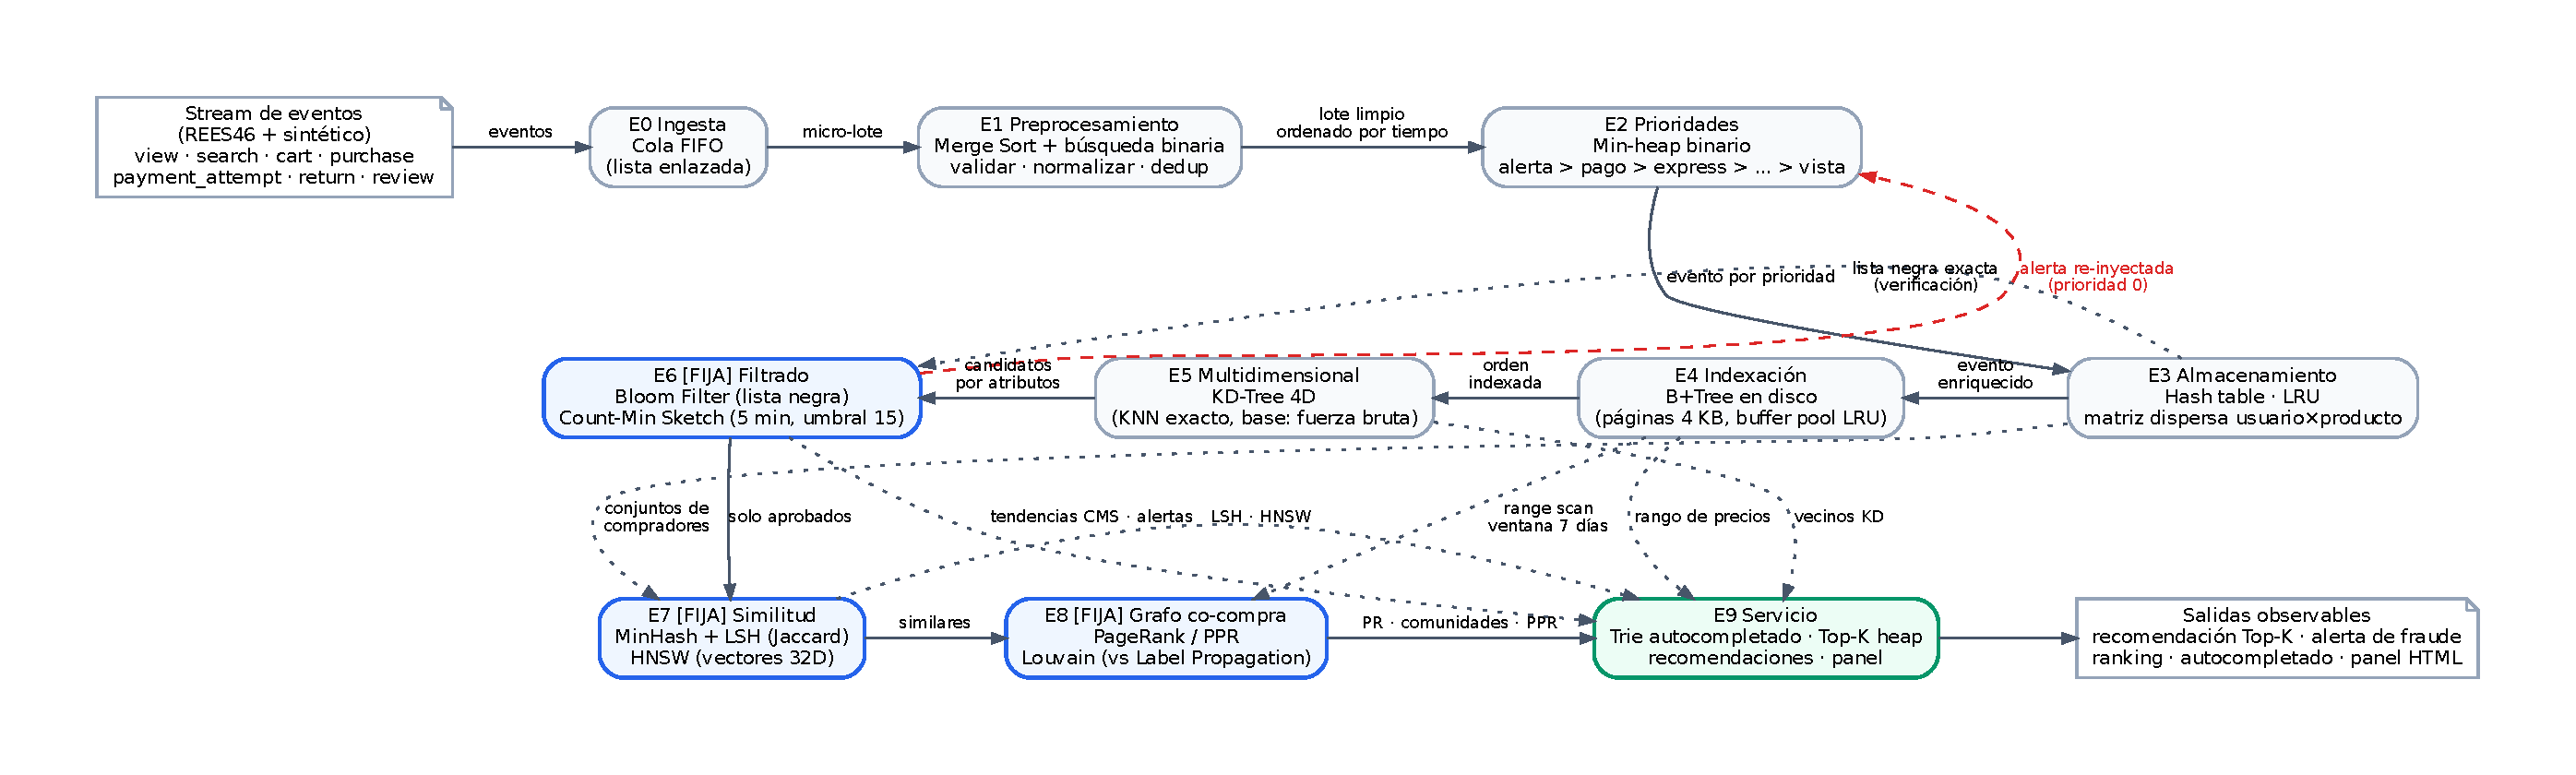
\includegraphics[width=\linewidth]{../diagrama_pipeline.pdf}
\caption{Arquitectura de 10 etapas. Flechas sólidas: flujo principal de cada evento; punteadas: salidas de una etapa consumidas por otra
(lista negra exacta, conjuntos de compradores, \emph{range scan} temporal, vecinos, tendencias); discontinua roja: realimentación de alertas
de fraude a la cola de prioridades con prioridad 0.}
\label{fig:arq}
\end{figure}
\vspace{-4pt}
El procesamiento es por \textbf{micro-lotes} (como Spark Structured Streaming): E0–E6 actúan evento a evento sobre cada lote y E7–E8, cuyo
costo es global, se recalculan cada 20 lotes con los datos que ya pasaron el filtro. La integración es verificable: el script
\texttt{scripts/demo.py} marca eventos concretos y registra lo que cada etapa hizo con ellos (Sección~\ref{sec:demo}).
Las etapas 0--5 se resumen en la Tabla~\ref{tab:base}; las etapas \textsc{fija} 6--8 se documentan en profundidad en la Sección~\ref{sec:inv}.

\begin{table}[H]
\centering\small
\caption{Etapas 0–5 y 9: función, estructura (implementación propia), complejidad y justificación frente a alternativas.}
\label{tab:base}
\begin{tabularx}{\linewidth}{@{}p{2.15cm}p{2.9cm}p{2.7cm}X@{}}
\toprule
\textbf{Etapa} & \textbf{Estructura} & \textbf{Complejidad} & \textbf{Función en el pipeline y justificación} \\
\midrule
E0 Ingesta & Cola FIFO con lista enlazada y capacidad máxima & enqueue/dequeue \Oh{1}; lote \Oh{b} & Buffer del stream con \emph{backpressure}. \texttt{list.pop(0)} es \Oh{n}; un arreglo circular exige capacidad fija. Entrega micro-lotes a E1. \\
E1 Preproceso & Merge Sort estable (runs de 16 con inserción) + búsqueda binaria & \Oh{b\log b} por lote; \Oh{\log W} por id & Valida y normaliza; categoría validada por búsqueda binaria; deduplica intra-lote (ordenar por \texttt{event\_id} + adyacentes) y entre lotes (búsqueda binaria en ventana ordenada de $W$=300K ids). Estable y sin peor caso \Oh{n^2} (Quicksort). Reordena por tiempo. \\
E2 Prioridades & Min-heap binario en arreglo, clave (prioridad, tiempo) & push/pop \Oh{\log n} & 9 clases: alerta $>$ pago $>$ express/premium $>$ estándar $>$ programada $>$ devolución $>$ carrito $>$ reseña $>$ vista. Lista ordenada: inserción \Oh{n}. El desempate por tiempo evita inanición dentro de cada clase. \\
E3 Almacén & Tabla hash (sondeo lineal, carga 0.7), LRU (hash + lista doble), matriz dispersa DOK$\to$CSR & \Oh{1} esperado; LRU \Oh{1}; \Oh{nnz} memoria & Producto, usuario, orden, pago y lista negra exacta. LRU para productos y resultados calientes (Zipf). Matriz usuario$\times$producto: densa costaría 8\,GB a $10^5\!\times\!10^4$. Enriquece el evento y alimenta E6, E7 y E9. \\
E4 Índice disco & B+Tree con páginas de 4\,KB en archivo + \emph{buffer pool} LRU (write-back) & \Oh{\log_B n} páginas; rango \Oh{\log_B n + k/B} & Índice temporal de órdenes (E8 lee la ventana de 7 días con \emph{range scan}) y de precios (E9). Fan-out $B\approx200$: altura 4 con $10^7$ claves vs.\ $\sim$24 de un AVL. \\
E5 Multidim. & KD-Tree 4D (mediana, dimensión de mayor dispersión, hojas de 32) + KNN fuerza bruta como base & construcción \Oh{n\log n}; consulta $\sim$\Oh{\log n} en $d$ bajo & Productos con atributos parecidos (precio, rating, popularidad, descuento) para cada vista; los productos son puntos (no rectángulos), por eso KD-Tree y no R-Tree. Resultados cacheados en LRU. \\
E9 Servicio & Trie con top-$K$ cacheado por nodo, Top-$K$ con min-heap de tamaño $K$ & autocompletar \Oh{|p|+K}; Top-$K$ \Oh{n\log K} & Autocompletado ponderado por ventas$\times$PageRank; recomendación por fusión de PPR (E8), LSH y HNSW (E7) y KD (E5); tendencias del CMS; panel HTML. \\
\bottomrule
\end{tabularx}
\end{table}

\section{Investigación avanzada: etapas 6–8}\label{sec:inv}
Para cada familia se resume fundamento, funcionamiento interno, complejidad, casos de uso, límites y \emph{trade-offs}, el paper original,
implementaciones de referencia (contra las que se validó la nuestra en \texttt{tests/}) y la evidencia empírica frente a la alternativa exacta o
más simple (Sección~\ref{sec:res}). Todas las estructuras están implementadas por el grupo en \texttt{src/ecostream/}.

\subsection{Filtrado probabilístico: Bloom Filter + Count-Min Sketch (E6)}
\textbf{Bloom Filter} (Bloom, 1970). \emph{Fundamento:} representar un conjunto $S$ con un arreglo de $m$ bits y $k$ funciones hash; aceptar
falsos positivos a cambio de memoria sublineal en el tamaño de las claves. \emph{Funcionamiento:} \texttt{add}$(x)$ enciende los bits
$g_i(x)$, $i=1..k$; \texttt{contains}$(x)$ responde \emph{posiblemente presente} si todos están encendidos y \emph{definitivamente ausente}
si alguno está apagado (sin falsos negativos). Usamos \emph{double hashing} $g_i(x)=h_1(x)+i\,h_2(x) \bmod m$ (Kirsch y Mitzenmacher, 2006),
que conserva la FPR asintótica con solo dos hashes de 64 bits (splitmix64 sobre BLAKE2b). \emph{Complejidad:} \Oh{k} por operación, independiente de
$n$; memoria $m=-n\ln p/(\ln 2)^2$ bits ($\approx$9.6 bits/elemento para $p=1\,\%$) con $k=(m/n)\ln 2$; FPR teórica $(1-e^{-kn/m})^k$.
\emph{Casos de uso:} listas negras, caché de “un solo acceso”, evitar lecturas a disco en LSM-trees (LevelDB, Cassandra), \emph{joins} distribuidos.
\emph{Límites:} no admite borrado (\emph{Counting Bloom} o \emph{Cuckoo filter}, Fan et al., 2014), exige estimar $n$ por adelantado (si se excede,
la FPR crece rápidamente; \emph{Scalable Bloom Filters}) y un positivo nunca es prueba. \emph{Referencias de implementación:} Guava \texttt{BloomFilter},
RedisBloom, \texttt{pybloom-live}.
\emph{Decisión en el pipeline:} el filtro contiene tokens de pago y dispositivos señalados ($n=50\,000$, $p=0.1\,\%$, 88\,KB). Un positivo
\textbf{no bloquea}: se verifica en la tabla hash exacta de E3 (decisión crítica); solo si se confirma se bloquea, y si no, se contabiliza como
falso positivo y la orden continúa. Así el Bloom ahorra la consulta exacta en el $\sim$99.9\,\% de pagos legítimos sin introducir bloqueos erróneos.

\textbf{Count-Min Sketch} (Cormode y Muthukrishnan, 2005). \emph{Fundamento:} resumen lineal de un \emph{stream} que estima frecuencias con error
aditivo acotado en memoria independiente del número de claves. \emph{Funcionamiento:} matriz $d\times w$ de contadores y $d$ hashes por pares
independientes; \texttt{update}$(x,c)$ suma $c$ en $C[i,h_i(x)]$ para cada fila y $\hat f(x)=\min_i C[i,h_i(x)]$. \emph{Garantía:} con
$w=\lceil e/\varepsilon\rceil$ y $d=\lceil\ln(1/\delta)\rceil$, $f(x)\le\hat f(x)\le f(x)+\varepsilon N$ con probabilidad $\ge1-\delta$ (nunca subestima).
\emph{Complejidad:} \Oh{d} por operación; memoria \Oh{wd}. \emph{Casos de uso:} \emph{heavy hitters}, tendencias, detección de DDoS y de
velocidad de transacciones, conteos aproximados en bases columnares. \emph{Límites:} el error es relativo a $N$ (malo para claves raras),
sesgo positivo (Count Sketch de Charikar et al.\ es insesgado; \emph{conservative update} reduce la sobreestimación). \emph{Referencias:}
RedisBloom (CMS), Apache DataSketches, \texttt{stream-lib}.
\emph{Decisión en el pipeline (clave, ventana y umbral exigidos):} \textbf{clave} = \texttt{payment\_token} y \texttt{device\_id} de cada intento de
pago; \textbf{ventana} deslizante de 5 minutos implementada como anillo de 5 sub-sketches de 60\,s ($\varepsilon=5\cdot10^{-4}$, $\delta=10^{-3}$);
\textbf{umbral} = más de 15 intentos en la ventana (un cliente legítimo hace 1–3). Al superarlo se genera una alerta que (i) se re-inyecta en el heap
con prioridad 0, (ii) agrega token y dispositivo al Bloom y a la lista negra exacta y (iii) se muestra en el panel. Un segundo CMS (ventana de 1\,h)
cuenta compras por producto y alimenta las tendencias de E9.

\subsection{Similitud de conjuntos: MinHash + LSH (E7)}
\emph{Fundamento} (Broder, 1997; Indyk y Motwani, 1998): para una permutación aleatoria $\pi$ del universo, $\Pr[\min\pi(A)=\min\pi(B)]=J(A,B)$.
Con $k$ permutaciones (aproximadas por hashes universales $h_i(x)=(a_ix+b_i)\bmod(2^{31}-1)$) la fracción de coincidencias estima $J$ con error estándar
$\sqrt{J(1-J)/k}$. \emph{LSH por bandas:} la firma se divide en $b$ bandas de $r$ filas y dos conjuntos son candidatos si coinciden en una banda completa:
$\Pr[\text{candidato}]=1-(1-J^r)^b$, una curva S con umbral $\approx(1/b)^{1/r}$. \emph{Complejidad:} firmas \Oh{k|A|} por conjunto; índice \Oh{nb};
consulta \Oh{b\log n+|C|\,k} frente a \Oh{n\,\bar{|A|}} de la fuerza bruta. Nuestra implementación guarda por banda un arreglo ordenado de claves de 64 bits
y responde con búsqueda binaria (\texttt{searchsorted}), y construye el índice por bloques sin materializar la matriz de firmas (10M conjuntos en $\sim$2.6\,GB).
\emph{Casos de uso:} casi-duplicados web, deduplicación de catálogos, \emph{item-item} colaborativo, plagio. \emph{Límites:} solo Jaccard; elegir $(b,r)$
fija el compromiso recall/candidatos; conjuntos muy pequeños tienen estimaciones ruidosas. \emph{Referencias:} \texttt{datasketch} (Python), Spark MLlib
\texttt{MinHashLSH}; Leskovec et al.\ (2020, cap.~3). \emph{Selección frente a SimHash} (Charikar, 2002): la señal de comportamiento es un conjunto binario
(usuarios que interactuaron con el producto), cuya similitud natural es Jaccard; SimHash aproxima coseno sobre vectores ponderados. \emph{Parámetros:}
$k=64$, $b=32$, $r=2$ (umbral 0.18), elegidos con el experimento de la Fig.~\ref{fig:lsh}: en este dominio la Jaccard producto–producto rara vez supera 0.3, y
la configuración típica $16\times4$ (umbral 0.5) recuperaba menos del 10\,\% de los vecinos reales del pipeline.

\subsection{ANN vectorial: HNSW (E7)}
\emph{Fundamento} (Malkov y Yashunin, 2020): grafos de mundo pequeño navegables más una jerarquía tipo \emph{skip list}. \emph{Funcionamiento:} cada
vector recibe un nivel $l=\lfloor-\ln U\cdot m_L\rfloor$, $m_L=1/\ln M$; las capas altas son “autopistas” con pocos nodos y la capa 0 contiene a todos.
La inserción baja voraz hasta $l$ y en cada capa ejecuta \texttt{search\_layer} con $ef_c$ candidatos, elige $M$ vecinos con la \textbf{heurística de
diversidad} (un candidato se acepta si está más cerca del nuevo nodo que de los ya elegidos; preserva puentes entre clústeres) y poda los vecinos que
exceden $M_{max}$. La consulta repite el descenso y explora la capa 0 con $ef\ge k$. \emph{Complejidad:} construcción \Oh{n\log n}, consulta
$\sim$\Oh{\log n} empírica, memoria \Oh{n(d+M)}. \emph{Casos de uso:} búsqueda semántica, recomendación por \emph{embeddings}, RAG.
\emph{Límites:} aproximado (recall $<1$ si $ef$ es bajo), memoria del grafo, borrado costoso, construcción cara en Python.
\emph{Referencias:} \texttt{hnswlib}, FAISS \texttt{IndexHNSWFlat}; en ANN-Benchmarks (Aumüller et al., 2020) los métodos basados en HNSW dominan el frente
recall–QPS. \emph{Selección frente a IVF y M-Tree/VP-Tree:} el catálogo crece con inserciones incrementales (HNSW no requiere reentrenar centroides como IVF,
Jégou et al., 2011) y el espacio de \emph{embeddings} normalizados es euclidiano (equivalente a coseno), por lo que no se necesita un índice métrico general.
El KD-Tree de E5 se mantiene para 4 dimensiones: en 32D visita casi todas las hojas (Fig.~\ref{fig:sim}), evidencia directa de la maldición de la dimensionalidad.

\subsection{Ranking de influencia: PageRank y Personalized PageRank (E8)}
\emph{Fundamento} (Brin y Page, 1998): la importancia de un nodo es la probabilidad estacionaria de un caminante aleatorio que sigue aristas con probabilidad
$d=0.85$ y se teletransporta con $1-d$. En el grafo de co-compra ponderado, $P_{ij}=w_{ij}/s_i$ y $r_{t+1}=d\,P^\top r_t+(d\,r_{\text{colg}}+1-d)\,v$.
\emph{Funcionamiento:} iteración de potencias hasta $\|r_{t+1}-r_t\|_1<10^{-9}$; cada iteración es un producto matriz dispersa–vector \Oh{m} (implementado con
\texttt{np.bincount}); converge geométricamente con razón $d$. \emph{Personalized PageRank} (Haveliwala, 2002) usa $v$ concentrado en las semillas (carrito y
compras del usuario) y mide afinidad con ellas: es la señal principal del recomendador. \emph{Límites:} en grafos no dirigidos PageRank está muy
correlacionado con el grado; es costoso recalcular PPR por usuario (se cachea en LRU). \emph{Referencias:} \texttt{networkx.pagerank} (nuestra
implementación coincide con un error $<10^{-6}$ en \texttt{tests/}), igraph, Spark GraphX. \emph{Alternativa simple:} ranking por grado ponderado.

\subsection{Comunidades: Louvain frente a Label Propagation (E8)}
\emph{Fundamento:} maximizar la modularidad $Q=\sum_c\left[L_c/m-(S_c/2m)^2\right]$ (Newman, 2006). \textbf{Louvain} (Blondel et al., 2008), el algoritmo
elegido, alterna (1) movimientos locales: cada nodo pasa a la comunidad vecina con mayor ganancia $\Delta Q\propto k_{i,c}-S_c k_i/2m$ hasta que no hay mejora, y
(2) agregación de cada comunidad en un super-nodo; se repite por niveles. Complejidad empírica $\sim$\Oh{m\log n}, memoria \Oh{n+m}.
\textbf{Label Propagation} (Raghavan et al., 2007), la alternativa más simple: cada nodo adopta la etiqueta de mayor peso entre sus vecinos, en orden aleatorio,
hasta que no hay cambios; \Oh{m} por iteración, sin función objetivo y sensible al orden. Girvan–Newman se descartó por su costo \Oh{m^2n}.
\emph{Límites:} límite de resolución de la modularidad (Fortunato y Barthélemy, 2007) y comunidades internamente desconectadas en Louvain, que Leiden
(Traag et al., 2019) corrige; LPA puede colapsar en una comunidad gigante y varía entre ejecuciones. \emph{Referencias:} \texttt{networkx} (\texttt{louvain\_communities}),
\texttt{python-louvain}, igraph \texttt{community\_multilevel}, \texttt{leidenalg}; nuestra modularidad coincide con la de networkx y nuestro Louvain alcanza
su $Q$ en \texttt{tests/}.


\section{Diseño e integración}\label{sec:diseno}
\textbf{Recorrido de un evento.} (1) E0 encola el evento en la FIFO; el consumidor extrae micro-lotes de tamaño variable (0.55–1.4$\times$5\,000, para simular
picos). (2) E1 normaliza, rechaza precios negativos o tipos desconocidos, marca precios faltantes y elimina duplicados (intra-lote por Merge Sort, entre lotes por
búsqueda binaria). (3) E2 inserta el lote en el heap; por \emph{tick} se atienden a lo más 5\,000 eventos (capacidad de servicio), así que en los picos esperan
las vistas y no los pagos. (4) E3 enriquece con el registro del producto (vía LRU), completa el precio faltante, actualiza el perfil, la matriz dispersa y la
orden. (5) E4 inserta la orden en el B+Tree temporal. (6) E5 obtiene vecinos por atributos para vistas y carritos. (7) E6 decide cada pago: Bloom$\to$verificación
exacta y CMS$\to$umbral; las alertas vuelven a E2 con prioridad 0 y el estado (aprobado/bloqueado) se propaga a la orden. (8) Cada 20 lotes, E7 reconstruye
MinHash+LSH con los conjuntos de usuarios por producto (solo compras aprobadas) y E8 lee del B+Tree las órdenes \textbf{aprobadas} de los últimos 7 días,
construye el grafo de co-compra y recalcula PageRank y Louvain. (9) E9 actualiza los pesos del Trie (ventas $\times$ PageRank) y responde.

\textbf{Puntuación de recomendaciones (E9).} Para un usuario con semillas $S$ (carrito, últimas compras y vistas), cada candidato $p$ recibe
$0.45\,\widehat{\mathrm{PPR}}_S(p)+0.30\,\hat J_{\mathrm{LSH}}(p)+0.15\,\cos_{\mathrm{HNSW}}(p)+0.03\,[p\in\mathrm{KD}]+0.07\,\widehat{\mathrm{PR}}(p)$
(cada término normalizado a $[0,1]$), se excluyen productos ya comprados y se seleccionan los $K$ mejores con un min-heap de tamaño $K$. Sin historial
(arranque en frío) se devuelven los productos de mayor PageRank. Cada recomendación lleva su explicación (qué fuentes la generaron).

\textbf{Decisiones de implementación.} (i) Todas las estructuras son propias; NumPy se usa para vectorizar núcleos numéricos (hashes del Bloom/CMS por lotes, distancias,
\texttt{bincount} de PageRank), y existen versiones escalares (evento a evento) del Bloom y del CMS que el pipeline usa en línea. (ii) El B+Tree es un índice en
disco real: los nodos se serializan en páginas de 4\,KB de un archivo y se leen/escriben a través del \emph{buffer pool} LRU de E3, lo que permite medir lecturas de página.
(iii) Las etapas globales (E7, E8) son incrementales por micro-lotes y no por evento, ya que Louvain o la reconstrucción del LSH por evento serían
\Oh{m} por evento. (iv) Corrección verificada con 14 pruebas (\texttt{tests/test\_structures.py}) contra \texttt{dict}, \texttt{heapq}, \texttt{bisect},
fuerza bruta y \texttt{networkx}.


\section{Metodología experimental}\label{sec:metodo}
\textbf{Plataforma.} Intel Xeon @ 2.30\,GHz, 2 vCPU, 7.8\,GB de RAM, Linux 6.18, Python 3.13.16, NumPy 2.5.3. \textbf{Semilla} global 42 (cada
tamaño usa $42+n$ para que los datos sean distintos pero reproducibles). Los experimentos se ejecutaron en dos colas paralelas, una por núcleo, y los de
$10^7$ de forma secuencial (\texttt{experiments/run\_all.sh}).

\textbf{Tamaños.} Para cada estructura base y cada etapa \textsc{fija} se generaron datasets de $10^3$, $10^4$, $10^5$, $10^6$ y $10^7$ elementos (operaciones,
claves, conjuntos, vectores, aristas o eventos según la estructura). \textbf{Repeticiones:} una corrida de calentamiento estima $t$ y luego
$\text{reps}=\min(100,\max(r_{\min},\lfloor 60\,\mathrm{s}/t\rfloor))$, con $r_{\min}=3$ hasta $10^6$ y entre 1 y 3 en $10^7$; se reportan media y desviación
estándar. Con ello $10^3$–$10^4$ (y casi todo $10^5$) alcanzan 100 repeticiones; en $10^6$–$10^7$ se usan menos porque una sola corrida de una estructura en
Python puro dura de segundos a minutos y el presupuesto total de cómputo es de 2 vCPU. Cada fila de \texttt{experiments/results/*.csv} reporta su número real de
repeticiones. \textbf{Memoria:} corrida aparte con \texttt{tracemalloc} (memoria retenida por la estructura y pico durante la operación; NumPy registra sus
\emph{buffers}); en $10^7$, donde \texttt{tracemalloc} multiplica el tiempo 3–5$\times$, se usa la herramienta equivalente: RSS de \texttt{psutil} en un proceso hijo
(actual) y \texttt{ru\_maxrss} (pico). \textbf{Escalabilidad:} se grafica en log-log y se ajusta $t=a\,n^{b}$ por mínimos cuadrados; la pendiente $b$ se contrasta
con la complejidad esperada (1 para lineal, $\approx$1.05–1.1 para $n\log n$ en este rango, 2 para cuadrática, $\approx$0 para logarítmica).
\textbf{Calidad:} FPR empírica sobre $n$ claves ausentes; error del CMS contra un \texttt{Counter} exacto; recall@10 de LSH y HNSW contra fuerza bruta;
modularidad, número/tamaño de comunidades, estabilidad (NMI media entre pares de semillas) y NMI contra las comunidades plantadas.


\section{Resultados}\label{sec:res}
\subsection{Demostración de punta a punta}\label{sec:demo}
Con 300\,000 eventos (\texttt{scripts/demo.py}, salida completa en \texttt{docs/demo\_output.txt}) el pipeline procesa el stream a $\sim$12\,000 eventos/s;
con 1M eventos, a 7\,600 eventos/s, y con 10M, a 7\,674 eventos/s (Tabla~\ref{tab:pipe}). Ejemplos de recorridos registrados por el trazador:
(i) una \textbf{compra express} entra en la FIFO, E1 la valida y verifica por búsqueda binaria que no es duplicada, E2 la inserta con prioridad 2 y sale del heap sin
esperar, E3 la enriquece (producto, precio), E4 indexa su orden en el B+Tree, E6 la aprueba, E7 la usa en los conjuntos de compradores, E8 la incorpora al grafo de la
ventana y E9 devuelve un Top-5 para el usuario; (ii) un \textbf{intento de pago} de una ráfaga supera el umbral del CMS, se bloquea y la alerta re-inyectada se atiende
con prioridad 0; (iii) un registro con precio negativo se rechaza en E1 y una re-entrega duplicada se elimina en E1. En ningún tamaño los pagos, alertas o compras
esperaron en el heap (0 \emph{ticks}); solo las vistas/búsquedas esperaron en los picos (0.47–0.66 \emph{ticks} en promedio). Los positivos del Bloom se
verificaron en la tabla hash antes de bloquear: 0 bloqueos erróneos.

\begin{table}[H]\centering\small
\caption{Pipeline completo (20\,000 productos, micro-lote 5\,000; 10\,000 en 10M). Costo por etapa en µs por elemento que la etapa procesa.}\label{tab:pipe}
\resizebox{\linewidth}{!}{\setlength{\tabcolsep}{4pt}
\begin{tabular}{@{}rrrrrrrrrrrrrr@{}}\toprule
Eventos & Procesados & s & ev/s & RSS GB & Órd. aprob./bloq. & Alertas & E0 & E1 & E2 & E3 & E4 & E5 & E6 \\\midrule
$10^4$ & 9\,996 & 1 & 10\,333 & 0.1 & 348 / 2 & 3 & 10 & 4 & 5 & 5 & 4 & 56 & 91 \\
$10^5$ & 99\,901 & 9 & 11\,551 & 0.2 & 3\,480 / 17 & 3 & 5 & 5 & 5 & 5 & 4 & 37 & 99 \\
$10^6$ & 999\,061 & 132 & 7\,597 & 1.1 & 34\,808 / 146 & 20 & 7 & 15 & 7 & 7 & 5 & 37 & 78 \\
$10^7$ & 9\,990\,165 & 1302 & 7\,674 & 4.5 & 348\,074 / 1405 & 200 & 15 & 15 & 11 & 10 & 5 & 38 & 63 \\
\bottomrule\end{tabular}}
\end{table}
\vspace{-6pt}
La etapa más costosa por elemento es E7 (reconstrucción del LSH y, sobre todo, la construcción del HNSW de 20\,000 productos, 40\,s fijos de inicialización), seguida
por E6 (Bloom + dos CMS escalares por pago, 63–99\,µs) y E5 (KD-Tree, $\sim$37\,µs, mitigado por un LRU con 69\,\% de aciertos). E0–E4 cuestan 4–15\,µs por evento.

\subsection{Estructuras base (E0–E5, E9)}
\begin{figure}[H]\centering
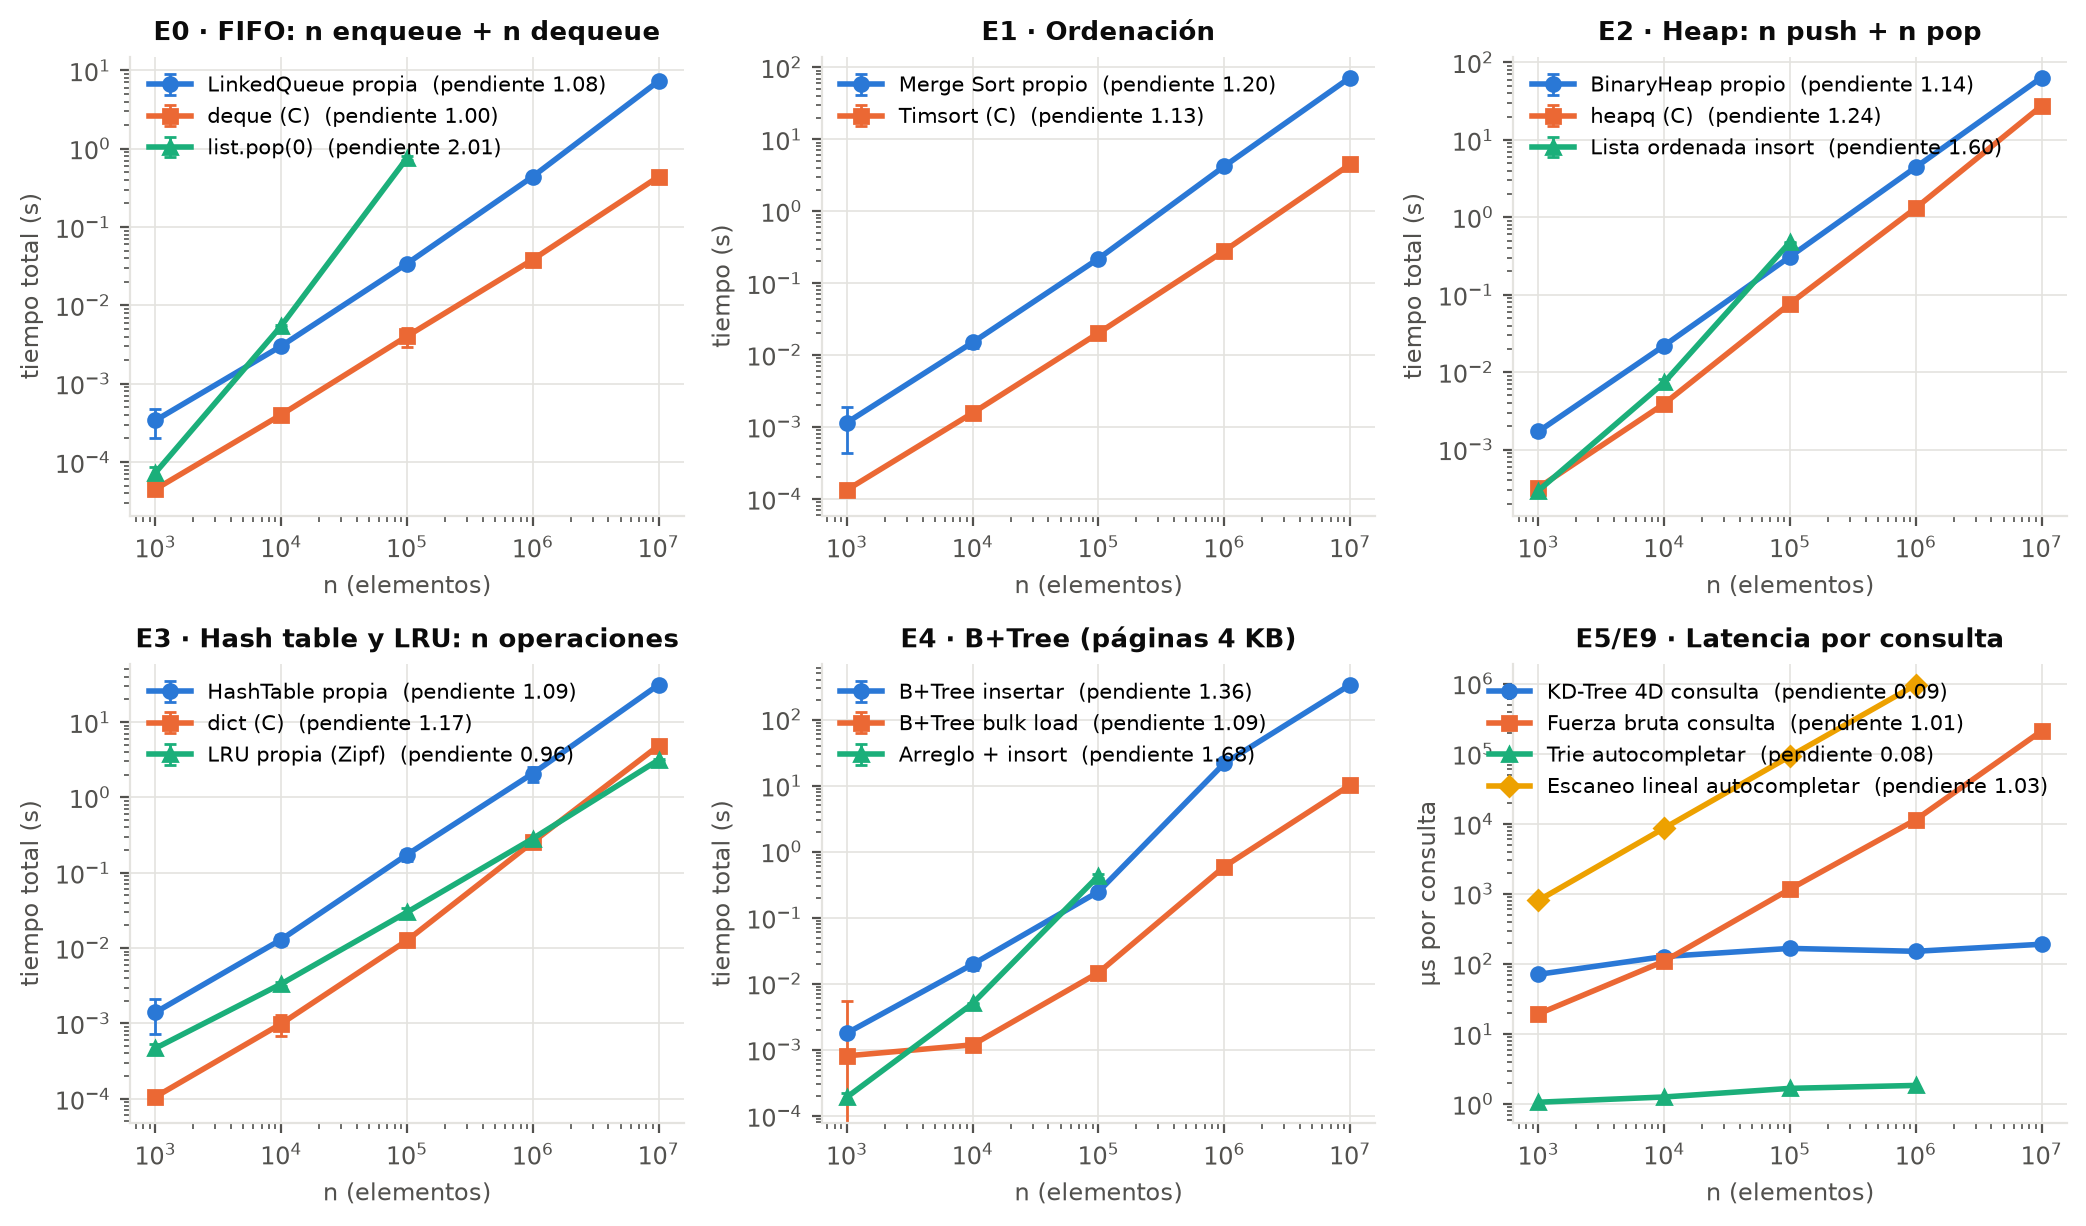
\includegraphics[width=\linewidth]{../../experiments/figures/fig_base_loglog.png}
\caption{Escalabilidad log-log (media $\pm$ desviación estándar) de las estructuras base frente a referencias en C y alternativas ingenuas; en la leyenda, la pendiente
ajustada $b$ de $t\propto n^b$ entre $10^3$ y el mayor tamaño medido ($10^7$ salvo las alternativas cuadráticas y el Trie).}\label{fig:base}
\end{figure}
\begin{table}[H]\centering
\caption{Pendiente ajustada $b$ ($t\propto n^b$, de $10^3$ al mayor tamaño medido) frente a la esperada; para latencias por consulta, $b\approx0$ indica costo sublineal.}\label{tab:slopes}
\setlength{\tabcolsep}{3.5pt}\footnotesize
\begin{tabular}{@{}lrl|lrl@{}}\toprule
Estructura / operación & $b$ & Esperada & Estructura / operación & $b$ & Esperada \\\midrule
LinkedQueue propia & 1.08 & 1 & Escaneo lineal autocompletar & 1.03 & 1 \\
deque (C) & 1.00 & 1 & Bloom insertar & 1.00 & 1 \\
list.pop(0) & 2.01 & 2 & set insertar & 1.13 & 1 \\
Merge Sort propio & 1.21 & $\approx$1.05-1.1 & Bloom consultar 2n & 1.01 & 1 \\
Timsort (C) & 1.13 & $\approx$1.05-1.1 & set consultar 2n & 1.15 & 1 \\
BinaryHeap propio & 1.15 & $\approx$1.05-1.1 & MinHash+LSH consulta & 0.06 & $\approx$0 \\
heapq (C) & 1.24 & $\approx$1.05-1.1 & Fuerza bruta Jaccard & 1.12 & 1 \\
Lista ordenada insort & 1.60 & 2 & HNSW consulta (ef=50) & 0.11 & $\approx$0 \\
HashTable propia & 1.09 & 1 & KNN exacto fuerza bruta & 1.06 & 1 \\
dict (C) & 1.17 & 1 & KD-Tree 32D & 0.95 & $\approx$1 \\
LRU propia (Zipf) & 0.96 & 1 & MinHash+LSH construir & 1.12 & 1 \\
B+Tree insertar & 1.36 & $\approx$1.05-1.1 & HNSW construir & 1.04 & $\approx$1.1 \\
B+Tree bulk load & 1.09 & 1 & PageRank & 1.07 & 1 \\
Arreglo + insort & 1.68 & 2 & Louvain & 1.22 & $\approx$1-1.2 \\
KD-Tree 4D consulta & 0.09 & $\approx$0-0.3 & Label Propagation & 1.22 & $\approx$1 \\
Fuerza bruta consulta & 1.01 & 1 & Grado ponderado & 0.51 & 0-1 \\
Trie autocompletar & 0.08 & 0 & & & \\
\bottomrule\end{tabular}
\end{table}
\vspace{-6pt}
Las pendientes confirman las complejidades esperadas (Tabla~\ref{tab:slopes}): FIFO propia 1.08 frente a 2.01 de \texttt{list.pop(0)}; Merge Sort 1.21 y heap 1.15
($n\log n$; algo por encima del 1.1 ideal por efectos de caché y asignación de memoria en $10^7$); tabla hash 1.09 (\Oh{1} por operación, 1.3–1.4 sondeos por operación con carga $\le$0.7); B+Tree \emph{bulk load} 1.09 (lineal) frente a 1.68 del
arreglo ordenado con \texttt{insort} (cuadrático por desplazamientos). El B+Tree con inserciones aleatorias tiene pendiente 1.36 porque desde $10^6$ claves
(7\,418 páginas) el árbol ya no cabe en el \emph{buffer pool} de 1\,024 páginas: cada inserción paga lecturas y escrituras de página reales (9.4M escrituras con
$10^7$ claves). Aun así, con $10^7$ claves la altura es 4 y una búsqueda puntual cuesta 1.7 lecturas de disco y 23\,µs; un rango de 10\,000 claves, 1.7\,ms. El
KD-Tree 4D responde KNN exacto en 0.15–0.19\,ms visitando 68–94 nodos tanto con $10^6$ como con $10^7$ puntos (pendiente 0.09), frente a 11\,ms y 211\,ms de la
fuerza bruta (1\,100$\times$ en $10^7$). El Trie responde autocompletado en 1–1.8\,µs independientemente de $n$ (pendiente 0.08) frente a 963\,ms del escaneo lineal con $10^6$ nombres.
Las referencias en C son 3–15$\times$ más rápidas en tiempo constante, como se espera de Python interpretado; la forma de las curvas es la misma.
\emph{Memoria pico} con $10^7$: FIFO 457\,MB, heap 1.29\,GB (tuplas), tabla hash 256\,MB (frente a 320\,MB de \texttt{dict}), KD-Tree 309\,MB y B+Tree 14\,MB en RAM
(282\,MB de páginas en disco). Límite: el Trie con $10^6$ nombres ocupa 1.7\,GB (4.3M nodos con su top-$K$ cacheado), por lo que $10^7$ nombres
($\approx$17\,GB) no cabe en 7.8\,GB y no se ejecutó; un catálogo real de comercio electrónico rara vez supera $10^6$ productos, y la alternativa sería un trie
comprimido (radix) o un FST.

\subsection{Filtrado probabilístico (E6)}
\begin{figure}[H]\centering
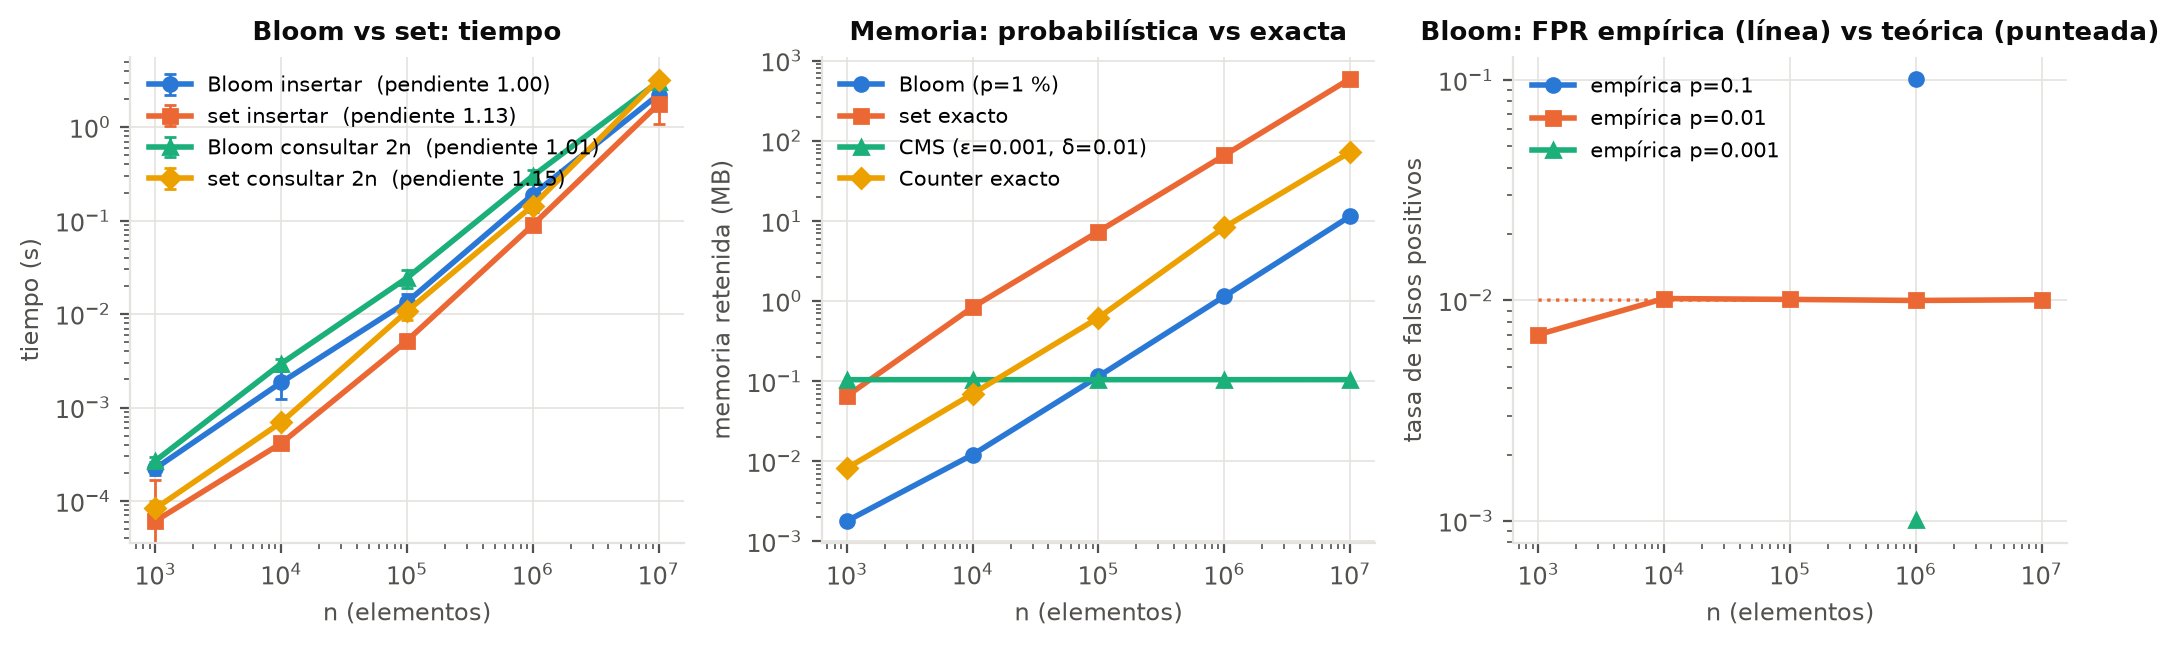
\includegraphics[width=\linewidth]{../../experiments/figures/fig_probabilisticas.png}
\caption{Bloom Filter frente a \texttt{set} (tiempo y memoria), CMS frente a \texttt{Counter} (memoria) y FPR empírica del Bloom frente a la teórica.}\label{fig:prob}
\end{figure}
\vspace{-6pt}
\begin{table}[H]\centering\small
\caption{Estructuras probabilísticas frente a la alternativa exacta (memoria retenida medida con tracemalloc; RSS en $10^7$).}\label{tab:prob}
\resizebox{\linewidth}{!}{\setlength{\tabcolsep}{4pt}
\begin{tabular}{@{}llllll@{}}\toprule
Comparación & $n$ & Construir (aprox./exacto) & Consultar $2n$ & Memoria (aprox./exacto) & Calidad \\\midrule
Bloom ($p$=1\,\%) vs \texttt{set} & $10^5$ & 13.46 ms / 5.19 ms & 24.36 ms / 10.71 ms & 118 KB / 7.4 MB & FPR 1.011\,\% (teórica 1.004\,\%), FN = 0 \\
Bloom ($p$=1\,\%) vs \texttt{set} & $10^6$ & 189.92 ms / 89.68 ms & 300.52 ms / 144.64 ms & 1.1 MB / 65.8 MB & FPR 1.000\,\% (teórica 1.004\,\%), FN = 0 \\
Bloom ($p$=1\,\%) vs \texttt{set} & $10^7$ & 2.23 s / 1.77 s & 3.08 s / 3.24 s & 11.4 MB / 594.4 MB & FPR 1.008\,\% (teórica 1.004\,\%), FN = 0 \\
CMS ($\varepsilon$=0.001) vs \texttt{Counter} & $10^5$ & 4.34 ms / 6.60 ms & -- & 107 KB / 635 KB & err. medio 8, máx 35 ($\varepsilon N$=100); 100\,\% en cota; subestim. 0 \\
CMS ($\varepsilon$=0.001) vs \texttt{Counter} & $10^6$ & 57.39 ms / 122.94 ms & -- & 107 KB / 8.3 MB & err. medio 138, máx 380 ($\varepsilon N$=1000); 100\,\% en cota; subestim. 0 \\
CMS ($\varepsilon$=0.001) vs \texttt{Counter} & $10^7$ & 654.48 ms / 2.05 s & -- & 107 KB / 72.3 MB & err. medio 1505, máx 40991 ($\varepsilon N$=9997); 100\,\% en cota; subestim. 0 \\
\bottomrule\end{tabular}}
\end{table}
\vspace{-6pt}
El Bloom Filter cumple la FPR teórica en todos los tamaños (1.008\,\% medida frente a 1.004\,\% teórica con $10^7$ claves; 0.101\,\% frente a 0.100\,\% con $p=0.1\,\%$) y
nunca da falsos negativos, con 9.6 bits por elemento: \textbf{11\,MB frente a 594\,MB} del \texttt{set} exacto con $10^7$ claves (52$\times$ menos). El tiempo es del mismo
orden que el del \texttt{set} (ambos lineales; el \texttt{set} es C nativo), así que la ventaja del Bloom es de \textbf{memoria}, no de velocidad, y por eso se usa como
filtro frente a la verificación exacta. El CMS ocupa 104\,KB constantes ($w=2\,719$, $d=5$) frente a 72\,MB del \texttt{Counter} con $\sim$950\,000 claves distintas;
nunca subestimó y el 100\,\% de las estimaciones quedó dentro de la cota $\varepsilon N$. El precio es el error aditivo: con $N=10^7$ el error medio es 1\,505 y el
error relativo en los 100 más frecuentes es 12\,\%; en el pipeline la ventana de 5 minutos mantiene $N$ pequeño y el error es despreciable frente al umbral de 15.

\subsection{Similitud aproximada (E7)}
\begin{figure}[H]\centering
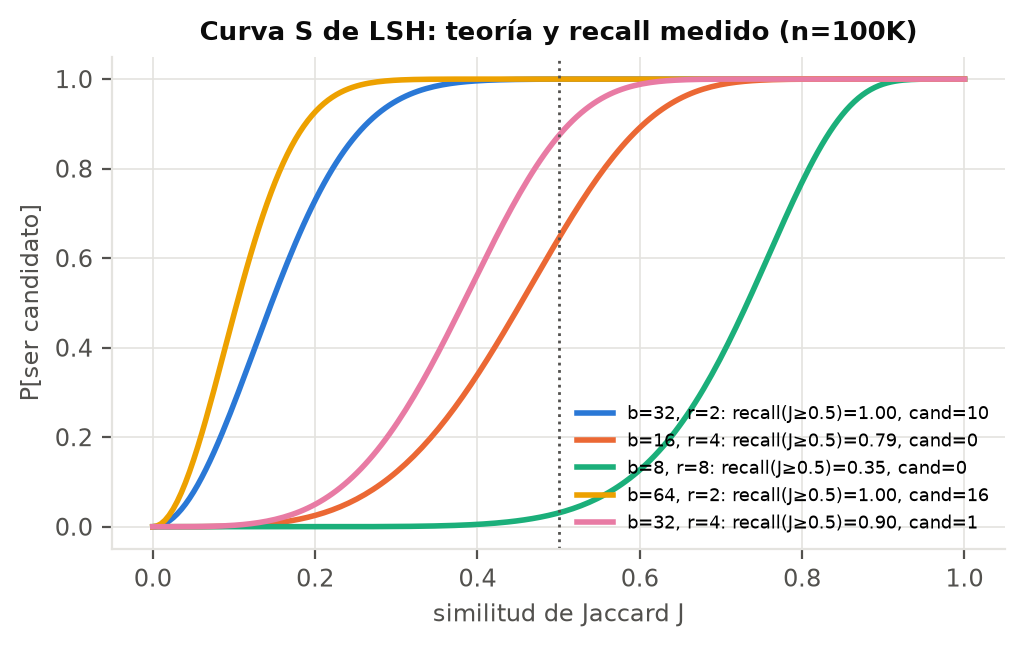
\includegraphics[width=0.36\linewidth]{../../experiments/figures/fig_lsh_curva.png}\hfill
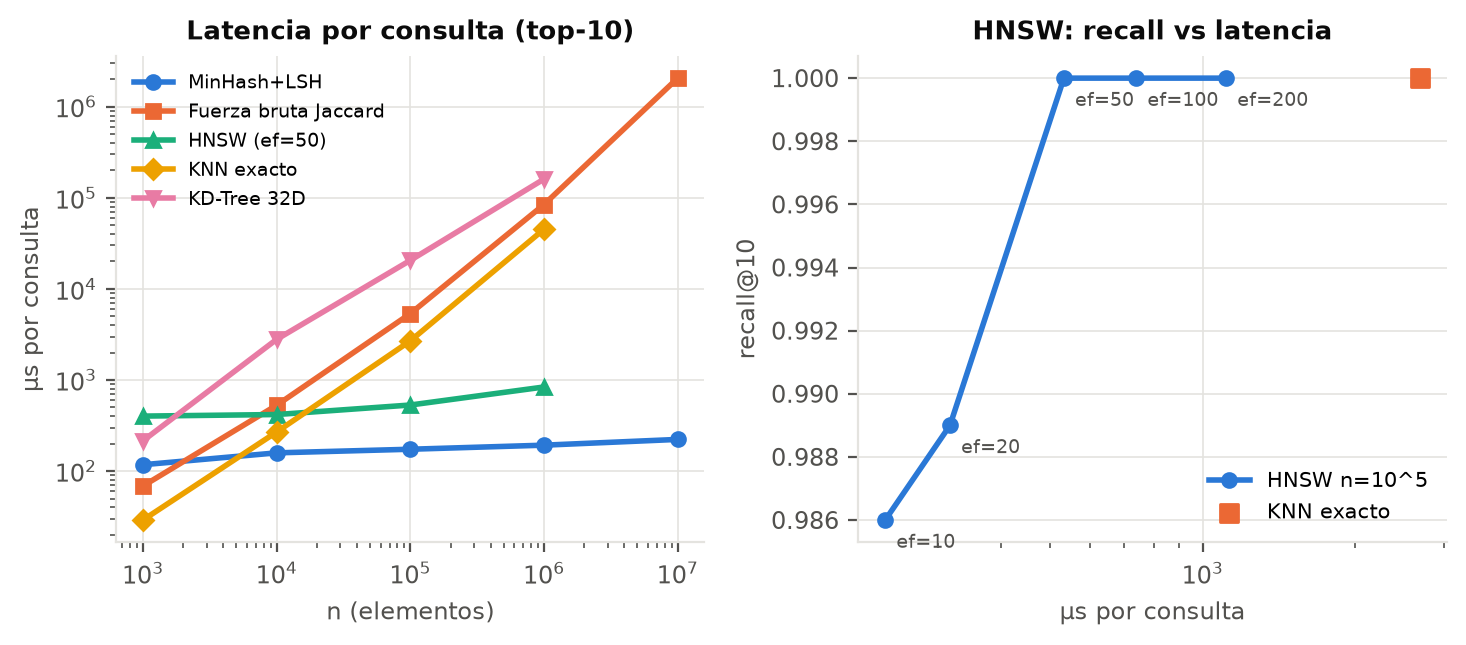
\includegraphics[width=0.63\linewidth]{../../experiments/figures/fig_similitud_ab.png}
\caption{Izquierda: curvas S teóricas de LSH y recall medido para varias $(b,r)$. Centro: latencia por consulta frente a $n$. Derecha: HNSW, recall@10 frente a latencia al variar $ef$ ($n=10^5$).}\label{fig:lsh}\label{fig:sim}
\end{figure}
\vspace{-6pt}
\begin{table}[H]\centering\small
\caption{Técnicas aproximadas frente a fuerza bruta / KNN exacto (consultas top-10).}\label{tab:sim}
\resizebox{\linewidth}{!}{\setlength{\tabcolsep}{4pt}
\begin{tabular}{@{}llrrrlll@{}}\toprule
Técnica & $n$ & Consulta aprox. & Exacto & Aceleración & Recall & Memoria (índice/datos) & Construcción \\\midrule
MinHash+LSH (32$\times$2) & $10^4$ & 0.16 ms & 0.5 ms & 3$\times$ & 1.00 (J$\ge$0.5) & 3.7 MB / 471 KB & 117.39 ms \\
MinHash+LSH (32$\times$2) & $10^5$ & 0.17 ms & 5.4 ms & 31$\times$ & 1.00 (J$\ge$0.5) & 36.6 MB / 4.6 MB & 2.77 s \\
MinHash+LSH (32$\times$2) & $10^6$ & 0.19 ms & 84.4 ms & 438$\times$ & 1.00 (J$\ge$0.5) & 366.2 MB / 45.8 MB & 30.64 s \\
MinHash+LSH (32$\times$2) & $10^7$ & 0.22 ms & 2\,057.7 ms & 9\,231$\times$ & 1.00 (J$\ge$0.5) & 2.40 GB / 457.8 MB & 232.62 s \\
HNSW ($M$=16, $ef$=50) & $10^4$ & 0.42 ms & 0.3 ms & 0.6$\times$ & 1.000 (@10) & 4.7 MB / 1.2 MB & 29.08 s \\
HNSW ($M$=16, $ef$=50) & $10^5$ & 0.53 ms & 2.7 ms & 5.1$\times$ & 1.000 (@10) & 48.9 MB / 12.2 MB & 296.74 s \\
HNSW ($M$=16, $ef$=50) & $10^6$ & 0.84 ms & 45.2 ms & 53.9$\times$ & 0.989 (@10) & 321.4 MB / 122.1 MB & 3324.31 s \\
\bottomrule\end{tabular}}
\end{table}
\vspace{-6pt}
\textbf{MinHash+LSH.} La consulta cuesta $\sim$0.2\,ms casi constante (pendiente 0.06) porque compara solo $\sim$10 candidatos; la fuerza bruta crece linealmente
(84\,ms en $10^6$ y 2.1\,s por consulta en $10^7$): \textbf{$\sim$9\,000$\times$ más rápido en $10^7$ con recall 1.0} para los vecinos con $J\ge0.5$. El recall sobre el top-10 completo
es 0.15–0.25 porque, más allá de los casi-duplicados, los vecinos tienen $J\approx0$ y LSH está diseñado para no verlos. El costo es la memoria: el índice ocupa
2.4\,GB frente a 458\,MB de los conjuntos en $10^7$ y se construye en 233\,s. La curva S (Fig.~\ref{fig:lsh}) muestra el compromiso: $16\times4$ (umbral 0.5) pierde 21\,\%
de los vecinos con $J\ge0.5$; $8\times8$, el 65\,\%; $32\times2$ los recupera todos con 10 candidatos y $64\times2$ con 16.
\textbf{HNSW.} Con $10^6$ vectores de 32 dimensiones responde en 0.84\,ms con recall@10 = 0.989, frente a 45\,ms del KNN exacto (54$\times$); con $10^5$, $ef=10$ da 0.986
en 0.24\,ms y $ef\ge50$ da recall 1.0. La construcción es el cuello de botella en Python (2.5–3.3\,ms por inserción; 55 minutos para $10^6$): con $10^7$ serían
$\sim$10 horas, por lo que el experimento de HNSW llega a $10^6$ (en C, \texttt{hnswlib} construye $10^7$ en minutos). El KD-Tree en 32D visita el 82\,\% de los nodos
y es más lento que la fuerza bruta (161\,ms frente a 45\,ms): evidencia directa de la maldición de la dimensionalidad que justifica usar KD-Tree solo en 4D (E5).

\subsection{Grafo: influencia y comunidades (E8)}
\begin{figure}[H]\centering
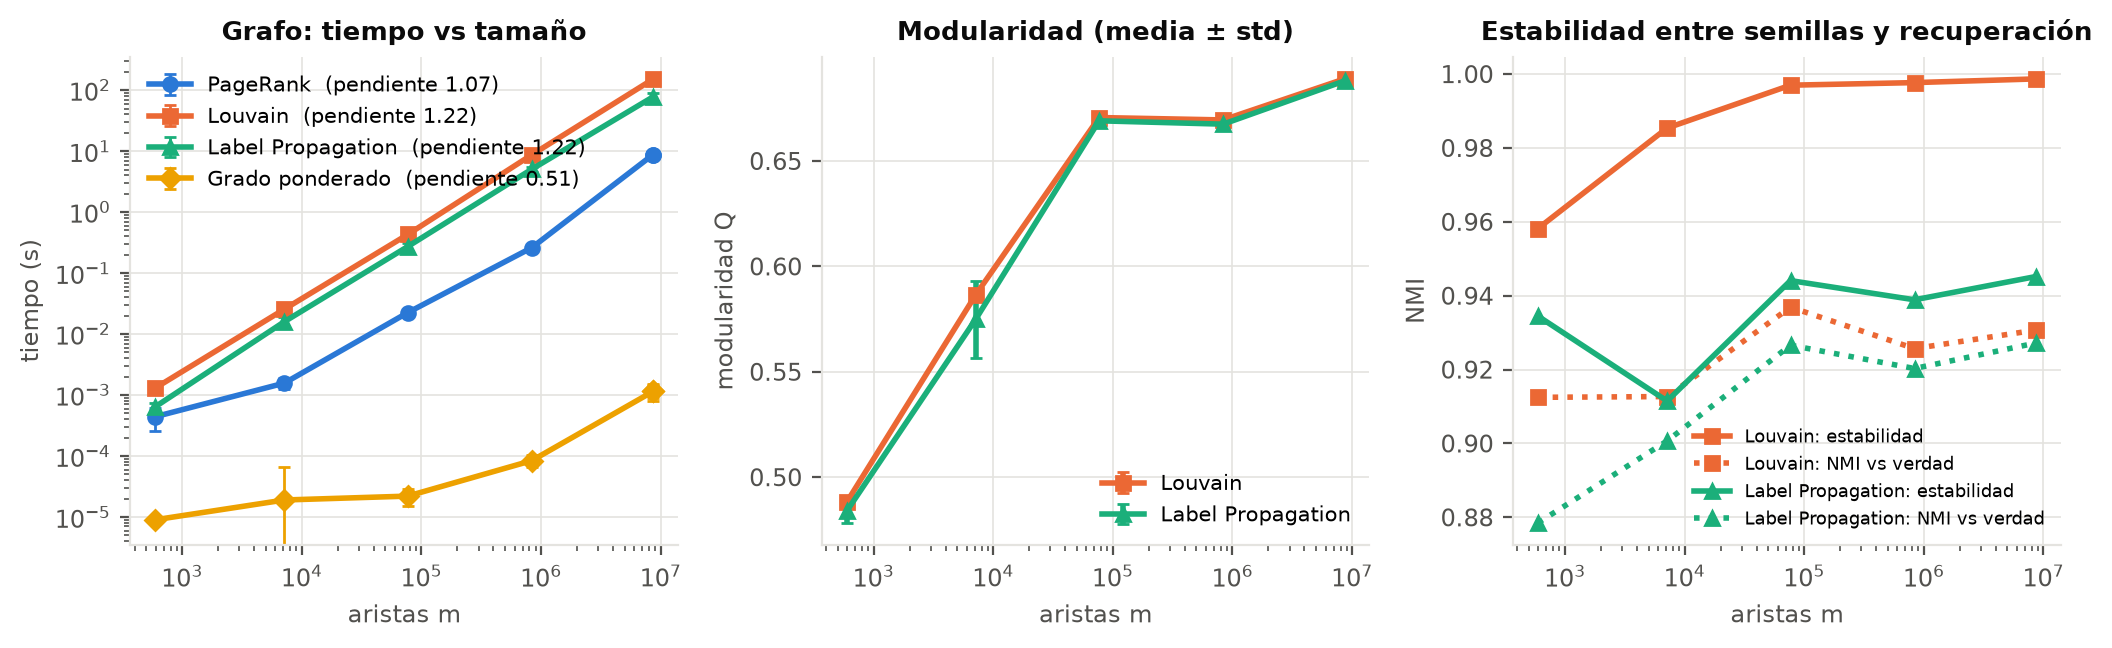
\includegraphics[width=\linewidth]{../../experiments/figures/fig_grafo.png}
\caption{Grafo con comunidades plantadas (70\,\% de aristas internas, grados Zipf, $n/8$ nodos): tiempo, modularidad (media $\pm$ std) y estabilidad/recuperación (NMI).}\label{fig:grafo}
\end{figure}
\vspace{-6pt}
\begin{table}[H]\centering\small
\caption{Louvain frente a Label Propagation en el mismo grafo (media sobre 10 semillas; 5 en $10^6$; 2 en $10^7$).}\label{tab:com}
\resizebox{\linewidth}{!}{\setlength{\tabcolsep}{4pt}
\begin{tabular}{@{}llllllll@{}}\toprule
Grafo ($n$ interacciones) & Alg. & Modularidad $Q$ & Tiempo & Nº comunidades & Mayor / mediana & Estabilidad (NMI) & NMI vs verdad \\\midrule
$10^4$ (7\,146 ar.) & Louvain & 0.5865 $\pm$ 0.0002 & 25.61 ms & 17 $\pm$ 0.0 & 310 / 54 & 0.985 & 0.913 \\
$10^4$ (7\,146 ar.) & LPA & 0.5750 $\pm$ 0.0183 & 15.96 ms & 19 $\pm$ 1.4 & 333 / 47 & 0.911 & 0.901 \\
$10^5$ (76\,778 ar.) & Louvain & 0.6706 $\pm$ 0.0000 & 429.72 ms & 56 $\pm$ 0.0 & 783 / 184 & 0.997 & 0.937 \\
$10^5$ (76\,778 ar.) & LPA & 0.6691 $\pm$ 0.0010 & 272.55 ms & 85 $\pm$ 2.2 & 805 / 133 & 0.944 & 0.927 \\
$10^6$ (835\,535 ar.) & Louvain & 0.6695 $\pm$ 0.0000 & 8.71 s & 167 $\pm$ 0.6 & 14\,491 / 431 & 0.998 & 0.926 \\
$10^6$ (835\,535 ar.) & LPA & 0.6675 $\pm$ 0.0005 & 5.05 s & 519 $\pm$ 12.7 & 15\,397 / 2 & 0.939 & 0.920 \\
$10^7$ (8\,641\,533 ar.) & Louvain & 0.6889 $\pm$ 0.0000 & 152.04 s & 553 $\pm$ 0.0 & 54\,995 / 1360 & 0.999 & 0.931 \\
$10^7$ (8\,641\,533 ar.) & LPA & 0.6880 $\pm$ 0.0000 & 77.88 s & 4\,722 $\pm$ 47.4 & 58\,061 / 2 & 0.945 & 0.927 \\
Co-compra real (15\,390 ar.) & Louvain & 0.7553 $\pm$ 0.0018 & 451.55 ms & 221 & 829 / 2 & 0.866 & -- \\
Co-compra real (15\,390 ar.) & LPA & 0.6303 $\pm$ 0.0111 & 190.62 ms & 848 & 372 / 3 & 0.860 & -- \\
\bottomrule\end{tabular}}
\end{table}
\vspace{-6pt}
\textbf{PageRank} converge en 38–42 iteraciones con costo lineal en $m$ (pendiente 1.07; 8.6\,s con 8.6M aristas). En un grafo no dirigido su correlación con el grado es
alta (Spearman 0.985; 95–99\,\% de coincidencia en el top-100), por lo que su valor diferencial está en la versión \textbf{personalizada}, que el ranking por grado no puede
dar: PPR desde el carrito es la señal con mayor peso del recomendador. \textbf{Comunidades:} en el grafo sintético ambos algoritmos alcanzan modularidades parecidas, pero
Louvain es \textbf{casi determinista} (NMI entre semillas 0.985–0.999 frente a 0.91–0.945; desviación de $Q\le2\cdot10^{-4}$ frente a hasta $2\cdot10^{-2}$ en LPA) y \textbf{no fragmenta}:
LPA deja miles de comunidades diminutas (mediana 2 nodos, 4\,722 comunidades en $10^7$ frente a 553). LPA es $\sim$2$\times$ más rápido. En el grafo de co-compra
\emph{real} del pipeline (1M eventos, 5\,681 productos, 15\,390 aristas), la diferencia es clara: Louvain $Q=0.755\pm0.002$ con 221 comunidades frente a LPA
$Q=0.630\pm0.011$ con 848; las comunidades de Louvain agrupan categorías complementarias plantadas (en la demo, la mayor reúne 91 laptops con 43 mouse, 42 teclados y 26 monitores).


\section{Conclusiones}
\begin{enumerate}[leftmargin=1.3em]
\item \textbf{La integración es el resultado.} Un evento atraviesa las 10 etapas y cada salida es la entrada real de otra: la lista negra exacta de E3 verifica los
positivos del Bloom de E6; las alertas del CMS vuelven a E2 con prioridad 0; solo las órdenes aprobadas por E6 entran, vía \emph{range scan} del B+Tree de E4, al grafo
de E8; el PPR de E8, el LSH/HNSW de E7 y el KD-Tree de E5 se fusionan en el Top-$K$ de E9. El pipeline procesa 10M eventos de punta a punta en Python puro.
\item \textbf{Las complejidades se cumplen empíricamente} (pendientes log-log de 1.0–1.2 para estructuras lineales y $n\log n$, 1.36 en el B+Tree por la E/S de disco, $\approx$0.1 para KD-Tree, Trie, LSH y HNSW,
$\approx$2 para las alternativas ingenuas). El B+Tree muestra el efecto que justifica su existencia: con $10^7$ claves, altura 4 y 1.7 lecturas de disco por búsqueda.
\item \textbf{Lo probabilístico cambia exactitud por memoria, con garantías medibles.} El Bloom cumple su FPR teórica con 52$\times$ menos memoria que un \texttt{set}
(sin ganar velocidad frente a un \texttt{set} nativo); el CMS usa memoria constante, nunca subestima y respeta $\varepsilon N$. Por eso ambos se usan como filtros
frente a una verificación exacta y no como decisión final.
\item \textbf{Lo aproximado cambia recall por velocidad.} MinHash+LSH responde $\sim$9\,000$\times$ más rápido que la fuerza bruta en $10^7$ sin perder vecinos con
$J\ge0.5$, pero sus parámetros deben ajustarse al dominio (la configuración típica 16$\times$4 fallaba con las similitudes bajas de co-compra). HNSW es 54$\times$ más rápido
que el KNN exacto en $10^6$ con recall 0.989; el KD-Tree, exacto y excelente en 4D, colapsa en 32D.
\item \textbf{Louvain frente a Label Propagation:} LPA es $\sim$2$\times$ más rápido, pero Louvain es estable entre ejecuciones, no fragmenta en miles de comunidades
diminutas y, en el grafo real de co-compra, logra mayor modularidad (0.755 frente a 0.630). PageRank aporta poco sobre el grado en grafos no dirigidos; su versión
personalizada es la que agrega valor.
\item \textbf{Límites y trabajo futuro:} la construcción de HNSW y el Trie de $10^7$ nombres no caben en el presupuesto de 2 vCPU/7.8\,GB en Python (se reportan hasta $10^6$);
el siguiente paso es un núcleo en C/Numba o \texttt{hnswlib}, Leiden en lugar de Louvain, \emph{Cuckoo filters} para permitir borrados en la lista negra, y validar el
pipeline con el CSV completo de REES46.
\end{enumerate}


\small
\section*{Referencias}
{\sloppy\setlength{\parindent}{0pt}\setlength{\parskip}{1.5pt}
\renewcommand{\baselinestretch}{0.95}\selectfont
Aumüller, M., Bernhardsson, E., \& Faithfull, A. (2020). ANN-Benchmarks: A benchmarking tool for approximate nearest neighbor algorithms. \emph{Information Systems, 87}, 101374. https://doi.org/10.1016/j.is.2019.02.006

Bloom, B. H. (1970). Space/time trade-offs in hash coding with allowable errors. \emph{Communications of the ACM, 13}(7), 422–426. https://doi.org/10.1145/362686.362692

Blondel, V. D., Guillaume, J.-L., Lambiotte, R., \& Lefebvre, E. (2008). Fast unfolding of communities in large networks. \emph{J. Stat. Mech.}, 2008(10), P10008. https://doi.org/10.1088/1742-5468/2008/10/P10008

Brin, S., \& Page, L. (1998). The anatomy of a large-scale hypertextual Web search engine. \emph{Computer Networks and ISDN Systems, 30}(1–7), 107–117. https://doi.org/10.1016/S0169-7552(98)00110-X

Broder, A. Z. (1997). On the resemblance and containment of documents. \emph{Compression and Complexity of Sequences}, 21–29. IEEE. https://doi.org/10.1109/SEQUEN.1997.666900

Charikar, M. (2002). Similarity estimation techniques from rounding algorithms. \emph{STOC '02}, 380–388. https://doi.org/10.1145/509907.509965

Cormen, T. H., Leiserson, C. E., Rivest, R. L., \& Stein, C. (2022). \emph{Introduction to algorithms} (4th ed.). MIT Press.

Cormode, G., \& Muthukrishnan, S. (2005). An improved data stream summary: The Count-Min sketch and its applications. \emph{Journal of Algorithms, 55}(1), 58–75. https://doi.org/10.1016/j.jalgor.2003.12.001

Fan, B., Andersen, D. G., Kaminsky, M., \& Mitzenmacher, M. (2014). Cuckoo filter: Practically better than Bloom. \emph{CoNEXT '14}, 75–88. https://doi.org/10.1145/2674005.2674994

Fortunato, S., \& Barthélemy, M. (2007). Resolution limit in community detection. \emph{PNAS, 104}(1), 36–41. https://doi.org/10.1073/pnas.0605965104

Haveliwala, T. H. (2002). Topic-sensitive PageRank. \emph{WWW '02}, 517–526. https://doi.org/10.1145/511446.511513

Indyk, P., \& Motwani, R. (1998). Approximate nearest neighbors: Towards removing the curse of dimensionality. \emph{STOC '98}, 604–613. https://doi.org/10.1145/276698.276876

Jégou, H., Douze, M., \& Schmid, C. (2011). Product quantization for nearest neighbor search. \emph{IEEE TPAMI, 33}(1), 117–128. https://doi.org/10.1109/TPAMI.2010.57

Kirsch, A., \& Mitzenmacher, M. (2006). Less hashing, same performance: Building a better Bloom filter. \emph{ESA 2006}, LNCS 4168, 456–467. https://doi.org/10.1007/11841036\_42

Leskovec, J., Rajaraman, A., \& Ullman, J. D. (2020). \emph{Mining of massive datasets} (3rd ed.). Cambridge University Press.

Malkov, Y. A., \& Yashunin, D. A. (2020). Efficient and robust approximate nearest neighbor search using hierarchical navigable small world graphs. \emph{IEEE TPAMI, 42}(4), 824–836. https://doi.org/10.1109/TPAMI.2018.2889473

Newman, M. E. J. (2006). Modularity and community structure in networks. \emph{PNAS, 103}(23), 8577–8582. https://doi.org/10.1073/pnas.0601602103

Raghavan, U. N., Albert, R., \& Kumara, S. (2007). Near linear time algorithm to detect community structures in large-scale networks. \emph{Physical Review E, 76}(3), 036106. https://doi.org/10.1103/PhysRevE.76.036106

REES46 (2019). eCommerce behavior data from multi category store [Dataset]. Kaggle. https://www.kaggle.com/datasets/mkechinov/ecommerce-behavior-data-from-multi-category-store

Samet, H. (2006). \emph{Foundations of multidimensional and metric data structures}. Morgan Kaufmann.

Traag, V. A., Waltman, L., \& van Eck, N. J. (2019). From Louvain to Leiden: Guaranteeing well-connected communities. \emph{Scientific Reports, 9}, 5233. https://doi.org/10.1038/s41598-019-41695-z
}
\end{document}
